% The entire content of this work (including the source code
% for TeX files and the generated PDF documents) by 
% Hongxiang Chen (nicknamed we.taper, or just Taper) is
% licensed under a 
% Creative Commons Attribution-NonCommercial-ShareAlike 4.0 
% International License (Link to the complete license text:
% http://creativecommons.org/licenses/by-nc-sa/4.0/).
\documentclass{article}

\usepackage{float}  % For H in figures
\usepackage{amsmath, amssymb} % For math
\usepackage{mathtools} % dcases*, see https://en.wikibooks.org/wiki/LaTeX/Advanced_Mathematics#The_cases_environment
\numberwithin{equation}{subsection} % have the enumeration go to the subsection level.
									% See:https://en.wikibooks.org/wiki/LaTeX/Advanced_Mathematics
\usepackage{graphicx}   % need for figures
\usepackage{cite} % For bibligraphy
\usepackage{fancyref} % For lazy reference \fref
\usepackage[unicode]{hyperref} % For hyperlink everything.
\usepackage{CJKutf8} % For Chinese characters
%\usepackage{ dsfont } % For double struck fonts
\usepackage{braket} 
\usepackage[T1]{fontenc}
\usepackage{listings}

\usepackage{amsthm}
\newtheorem{defi}{Definition}[section]
\newtheorem{thm}{Theorem}[section]
\newtheorem{lemma}{Lemma}[section]
\newtheorem{remark}{Remark}[section]
\newtheorem{prop}{Proposition}[section]
\newtheorem{coro}{Corollary}[section]
\theoremstyle{definition}
\newtheorem{ex}{Example}[section]

\usepackage{tensor}  % For tensor indices
\usepackage[all]{xy} % For drawing category diagrams
\usepackage{mathrsfs}

\title{Lectures on the Frontiers of Physics}
\date{2016-07-22}
\author{we.taper}
\begin{document}
\maketitle
\abstract{
    This is notes of lectures given by (assistant/)professors of physics in SUSTC,
    each talking about their own researches. Since they are generally boring
    (targeted at first/second year students), I omitted many of them.
}
\tableofcontents


\section{By JQ. He.}
\textbf{Thermal electrics}

\section{By Lang. Chen}
\label{sec:c.l}
Grow thin films.
\begin{itemize}
\item Rheed-Assited PLD/MBE. (Ray as an exmination).
\item 
orbital contral of electrons -> 
orbitronics -> Control of Spin orbital coupling.
\item
Multiferroics -> multiple order parameters, and the interaction
between them. E.g. $BiFeO_3$.
\item
Ferrotorodicity: Spontaneous Toroidal Momennt. Time and spacial
symmetries simultaneous broken.
\item
What is a iridates $Ir_2(X)O_4$, (e.g. $Sr_2RuO_4$) 
exactly in theoretical physics?
\item
$H_2S$: 200K superconductor?
\item
The Double Exchange effect of oxygem -> Half-metal, phase transition.
\end{itemize}

\section{By Alan}
\textbf{Photocatalysis}: $TiO_2$. Hongkong has $TiO_2$ spurred on
the keys.

\section{By Li, Huang}
\begin{itemize}
        \item Computational Physics
        \item Surface Dynamics
        \item Structural factor from 2D to 3D.
        \item Finding Order Amid the Chaos. amorphous -> spatially
                resolved distributed function.
        \item ?: What is genetically algorithm.
\end{itemize}
\textbf{Computational and theoretical studies of Surface dynamics}

\begin{itemize}
        \item Surface atoms is immersed in a very different environment
                compared with the bulk atoms.
        \item First-principle calculations
        \item DFT + LDA -> Conser equation
        \item Plane wave basis + Ultrasoft pseudopotentials to solve the
                Conser equation
        \item Continumm method ?
\end{itemize}

\section{By Junfen, Liu}
\begin{itemize}
        \item electronic transport in mesoscopic systems:
        \item Spintronics
        \item Graphene eletronics
        \item Superconductors etc.
\end{itemize}
\textbf{Quantum wire conductiing}
The conduction channel in quantum wire is quantized, with discrete value
of conductance.
\begin{itemize}
        \item $\lambda_F$ Fermi wavelength
        \item $L_m$ Momuntum relaxation length <-- impurities.
        \item $L_\phi$ Phase relaxation length <-- memory of phase,
                related to energy $\omega = E/\hbar$.
        \item $L$ Sample length
\end{itemize}
\begin{itemize}
        \item Ballistic transport: $L << L_m$ No scattering.
        \item Diffusive $L>L_m$, scattering, reduced transmission.
        \item Localization $L_m<<L<<L_\phi$ -> Prof. Haizhou Lu.
        \item Classical. (Omitted)
\end{itemize}
\textbf{Conductance}
No back-scattering $$ G = \frac{I}{V} = \frac{2e^2}{h}$$
Landauer formula $G = \frac{2e^2}{h}\cdot T$, $T$ is some coefficient
accounting for the back scattering, perhaps the transmission
probability.
In reality, $G=\sum_{\text{Different channels}}G_i$, 

We can turn the $G$ into resisivity: 
$$\text{Resistance}= \frac{h}{2e^2} + \frac{h}{2*e^2}\frac{R}{T}$$
$R+T=1$

\subsection{Resonate Transmission} (Omitted)

\subsection{Spintronics} Use the extra freedom of Spin. 

Spin field eletroncis: Datta and Das, Appl. Phys. Lett. 56, 665(1990)

GMR: 2007 Nobel prize in Physics.

Hall Effect (Omitted)
Spin Hall Effect: S. murakami, et.al. Science 301 1348(2004);


J. Sinova et.al. Phys.Rev.Lett. 92, 126603 (2004). (Omitted)

\subsection{Graphene} Carrier -> Relativistic Dirac fermions.
\textbf{Klein Paradox} 

\subsection{Josephson Junction} A phase difference could conduct
electricity in Superconductors.



\section{By Haizhou, Lu}
\subsection{Quantum Anomalous Hall Effect}
Requires strong magnetic field: $\approx 10$ Tesla.

Anomalous Hall Effect: Without magnetic field. $R_H = R_0 B+ R_A M$
where $M$ is the magnetic susceptibility.
Two-factors: SO coupling. Spin-dependent Hall Effect.

An excellent illustrations is found in \cite{Arxiv-Xiao}:
\begin{figure}[H]
    \centering
    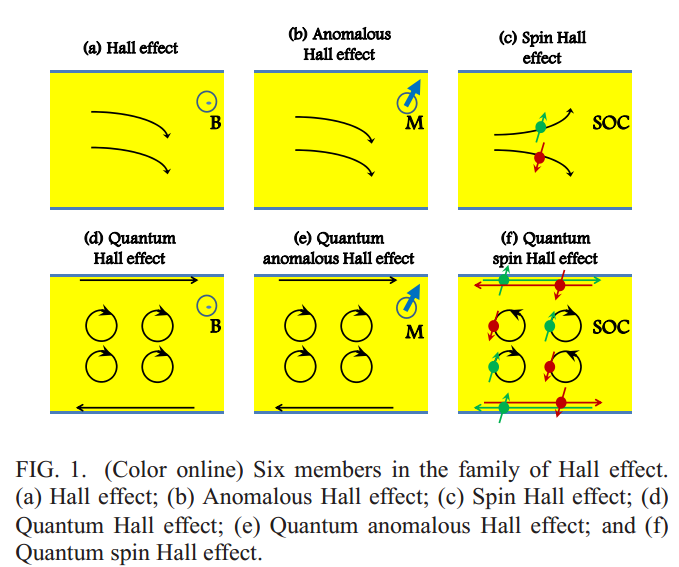
\includegraphics[width=0.8\linewidth]{pics/1}
    \caption{Illustration}
    \label{fig:Xiao Illustration}
\end{figure}

\section{By Kedong Wang}
Tunneling current $I\propto V e^{-2kz}$, where 
$k = \frac{\sqrt{2m\phi}}{\hbar}$, $\phi$ is the Work function.
$I$ is very sensitive to the distance $z$.

\subsection{Work function} $\phi$ characterize the obstruction
that prevents electron from escaping the sample.

\section{By Mingyuan Hunag}
Not insterested.

\section{By Wenkang Wong}
\subsection{Non-clone Theorem} We can easily see that there is no universal
copy operators in Quantum Mechanics.

\begin{proof}
We proove it by contradiction. Let $U$ be the copy operator. By definition,
we have
$$   U \ket{\psi}\ket{0} = \ket{\psi}\ket{\psi}$$
For any $\ket{\psi}$.
Then, let try copying the state $\ket{\psi} = \ket{0} + \ket{1}$. We have
\begin{align*}
    (\ket{0}+\ket{1})(\ket{0}+\ket{1}) &= U (\ket{0}+\ket{1})\ket{0} \\
    &= U (\ket{0}\ket{0} + \ket{1}\ket{0} ) \\
    &= \ket{0}\ket{0} + \ket{1}\ket{1} \\
\end{align*}
This is a contradiction.
\end{proof}
\begin{remark}
    We assume that the copier is universal. This might seems to be too
    strong. However, if we assume that the copyer only
    works for certain states $\ket{\phi}$, then with the knowledge
    of these certain states, we could in principle create an exact copy
    of these states. This copy ,in the sense of another instance of the
    same object, of original state should not be considered to be an
    copied version of the original state.
\end{remark}

\section{By Liyuan Zhang}
Not insterested.
\section{License}
The entire content of this work (including the source code
for TeX files and the generated PDF documents) by 
Hongxiang Chen (nicknamed we.taper, or just Taper) is
licensed under a 
\href{http://creativecommons.org/licenses/by-nc-sa/4.0/}{Creative 
Commons Attribution-NonCommercial-ShareAlike 4.0 International 
License}. Permissions beyond the scope of this 
license may be available at \url{mailto:we.taper[at]gmail[dot]com}.

\begin{thebibliography}{1}
    \bibitem{Arxiv-Xiao} \url{http://arxiv.org/abs/1508.07106v1}
\end{thebibliography}
\end{document}
